\section{数据分析与预处理}

\subsection{数据集来源与结构}

数据来源于Kaggle公开数据集
\emph{F1 Aerodynamic Stability and Porpoising (150k Samples)}。
原始数据包含约15万条样本，
经数据清洗后保留104,999条有效样本，
包含5个输入特征和1个目标变量。

\begin{table}[H]
\centering
\caption{数据字段描述}
\begin{tabular}{ccl}
\toprule
字段 & 类型 & 描述 \\
\midrule
speed\_kmh & float64 & 赛车时速 (km/h) \\
wing\_angle\_deg & float64 & 前翼角度 (°) \\
drs\_active & int (0/1) & DRS激活状态 \\
downforce\_n & float64 & 下压力 (N) \\
drag\_n & float64 & 空气阻力 (N) \\
stability\_index & float64 & 气动稳定性评分 (0--100) \\
\bottomrule
\end{tabular}
\end{table}

\subsection{描述性统计分析}

\begin{table}[H]
\centering
\caption{各特征描述性统计}
\begin{tabular}{lrrrrrr}
\toprule
特征 & 均值 & 标准差 & 最小值 & 中位数 & 最大值 & 偏度 \\
\midrule
speed\_kmh & 232.5 & 76.5 & 100.0 & 232.7 & 365.0 & $-$0.00 \\
wing\_angle\_deg & 20.0 & 8.7 & 5.0 & 20.0 & 35.0 & 0.00 \\
drs\_active & 0.30 & 0.46 & 0.0 & 0.0 & 1.0 & 0.88 \\
downforce\_n & 2392.4 & 1844.6 & 105.3 & 1842.5 & 8969.2 & 1.07 \\
drag\_n & 166.1 & 106.5 & 18.1 & 145.6 & 515.9 & 0.67 \\
stability\_index & 91.3 & 24.8 & 0.0 & 100.0 & 100.0 & $-$2.90 \\
\bottomrule
\end{tabular}
\end{table}

从统计表中可观察到：
speed\_kmh和wing\_angle\_deg近似对称分布（偏度$\approx 0$）；
downforce\_n和drag\_n呈右偏分布（偏度分别为1.07和0.67），
高值样本相对较少；
stability\_index呈严重左偏分布（偏度$=-2.90$），
大部分样本集中在高稳定性区域。

\subsection{数据不平衡分析}

稳定性分布存在严重的不平衡现象：

\begin{table}[H]
\centering
\caption{稳定性分级分布}
\begin{tabular}{lrrr}
\toprule
稳定性等级 & 评分范围 & 样本数 & 占比 \\
\midrule
严重不稳定 (severe) & [0, 30) & 9,563 & 6.38\% \\
中度不稳定 (moderate) & [30, 60) & 4,513 & 3.01\% \\
轻度不稳定 (mild) & [60, 95) & 6,895 & 4.60\% \\
稳定 (stable) & [95, 101) & 129,028 & 86.02\% \\
\bottomrule
\end{tabular}
\end{table}

稳定样本与不稳定样本的比例约为 6.15:1，
构成了典型的类不平衡问题。
高稳定性样本（$\geq 95$）占比86.02\%，
可能导致模型过度依赖数据量占优的稳定样本特征分布，
在低稳定性区域产生预测偏差。

针对不平衡问题，
采用类平衡加权策略：
\begin{equation}
    w_i = \frac{N}{K \cdot n_i}
\end{equation}
其中 $N$ 为总样本数，$K=4$ 为分级数，
$n_i$ 为第$i$级的样本数。
severe级权重3.92，moderate级权重8.31，
mild级权重5.44，stable级权重0.29。
该权重策略在模型训练损失函数中赋予低稳定性样本更高的优化优先级。

\subsection{数据预处理流程}

预处理包括以下步骤：
\begin{enumerate}
    \item \textbf{数据清洗}：检测并剔除缺失值和格式异常记录；
    \item \textbf{特征归一化}：对连续特征采用StandardScaler
        （用于XGBoost/Ridge/Random Forest；
        树模型（XGBoost、Random Forest）理论上不依赖特征缩放，
        此处为统一训练管线而保持预处理一致）和MinMaxScaler
        （用于神经网络模型）两种归一化策略；
    \item \textbf{数据集划分}：按7:1.5:1.5比例划分为训练集、
        验证集和测试集（random\_state=42）。
\end{enumerate}

\subsection{探索性数据分析}

\begin{figure}[H]
\centering
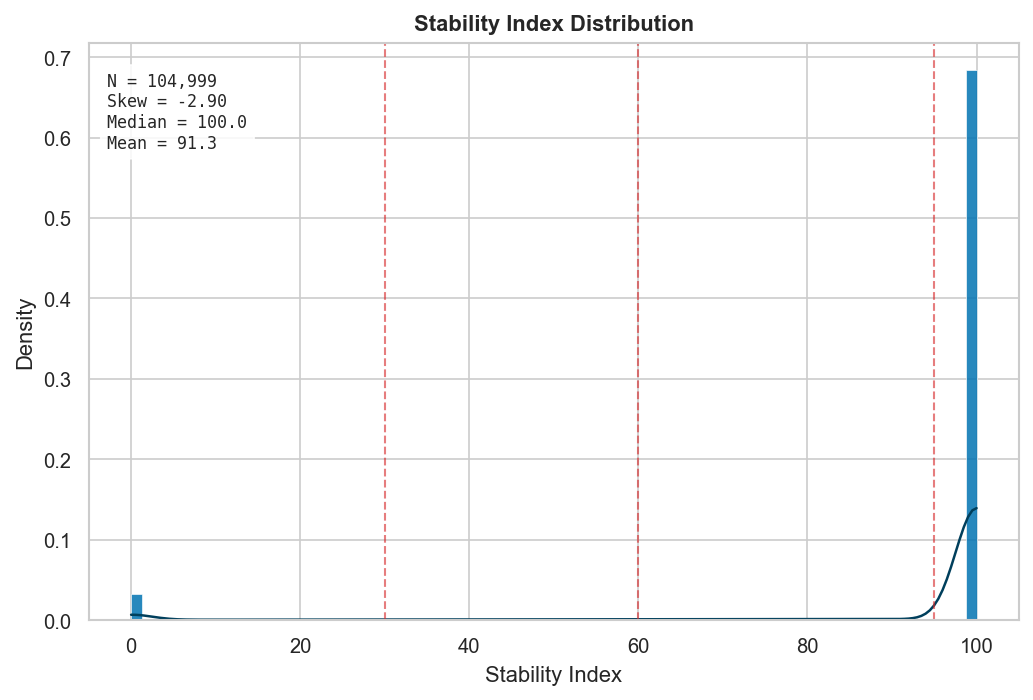
\includegraphics[width=0.78\textwidth]{figures/01_distribution.png}
\caption{各特征分布及稳定性评分分布直方图}
\label{fig:distribution}
\end{figure}

图\ref{fig:distribution}展示了6个变量的分布情况。
stability\_index呈现典型的"天花板效应"——
绝大多数样本集中在满分（100）附近，
这是后续代理模型在高稳定性区输出饱和的根本原因。

\begin{figure}[H]
\centering
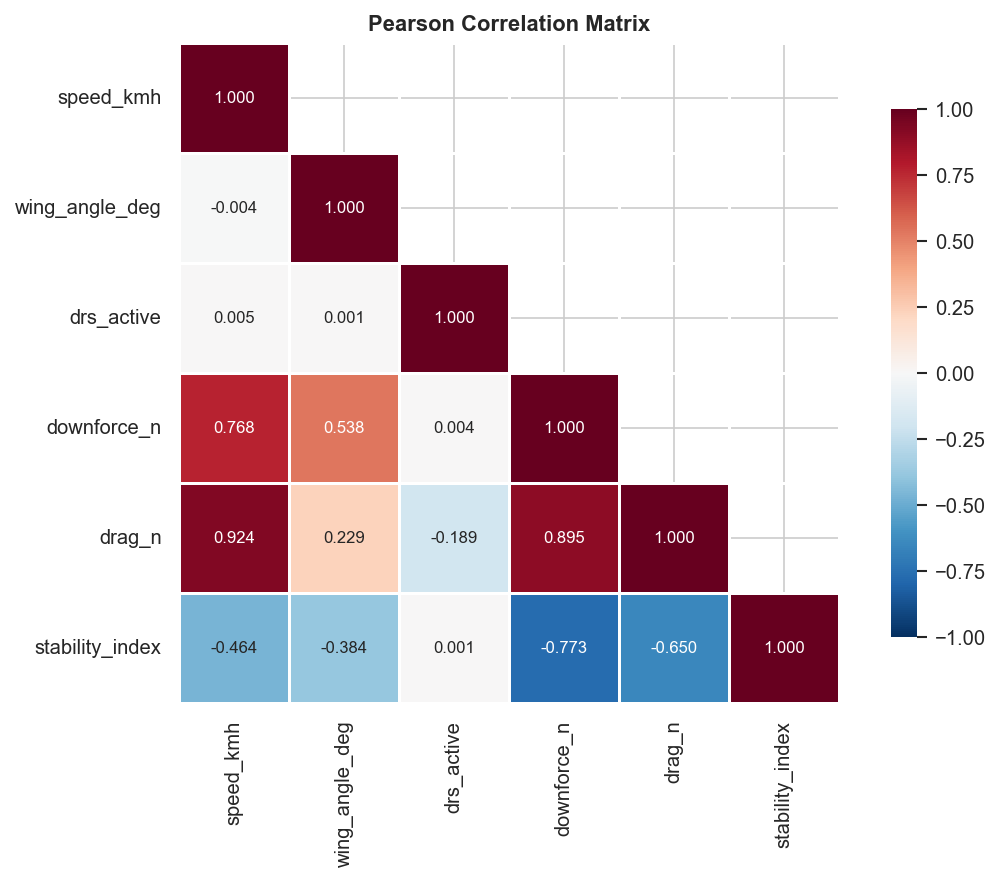
\includegraphics[width=0.75\textwidth]{figures/02_correlation.png}
\caption{特征间相关系数矩阵}
\label{fig:correlation}
\end{figure}

图\ref{fig:correlation}的相关系数矩阵揭示了关键的数据结构特征：
downforce\_n与stability\_index的相关性最强（Pearson r = $-$0.773，
Spearman $\rho = -0.617$）；
downforce\_n与drag\_n之间存在极强正相关（r = 0.895）；
wing\_angle\_deg与stability\_index的r = $-$0.384，
但控制downforce\_n后的偏相关系数仅为0.06，
表明翼角的影响几乎完全通过下压力实现中介传递。

值得注意的关键特征间耦合：
speed\_kmh与drag\_n的r = 0.924，
speed\_kmh与downforce\_n的r = 0.768，
这些强耦合关系解释了为什么高速工况下赛车同时面临高阻力和高下压力，
构成了气动设计的经典tradeoff。
